\chapter{Results}\label{chap:results}

The following section describes the experimental setup, the used and generated datasets as well as parameters to conclude with the experimental results achieved.

\section{Developped programs}
Many programs have been developped for the need of the present thesis. Early data exploration scripts have paved the way towards efficient highly parallel programs in both Rust and Python for data analysis, graph and embedding generation of ML and DL tested on different models and contexts. All the necessary concepts and methods have been introduced previously, so it is now time to present those main program in details.

\subsection{Mem2Graph}
The present report has already presented the \textit{Mem2Graph} program throughout the heap dump memory parsing algorithm, graph construction and embeddings. This program has been developped in Rust and is an active collaboration between the author and Clément Lahoche, another PhDTrack student at Passau. The program is available on GitHub at \url{https://github.com/passau-masterarbeit-2023/mem2graph}. 

The program is composed of several layers than bruild on top of each other. The first layer is dedicated into loading a RAW heap dump file with its annotation JSON file, performs some checks and prepare the data for further analysis. The next one performs the graph construction following the algorithms introduced in the Methods section. Another layer performs some annotations of the nodes. The final layer is more versatile and dependent on the input program parameters. For the need of this report, several pipelines of memgraph with and without embeddings haved been added, namely \texttt{graph} and \texttt{graph-with-embedding-comments}. The first pipeline doesn't perform any embedding and export the memory graph to a text file following the DOT format \cite{DotFormat15}. The second pipeline performs the same operations, but also exports the memory graph with the embeddings as comments in the DOT file. 

Since the prediction effort is focused on memory chunks, this embedding is generally called with the \texttt{--no-value-node} parameter, which transform the memory graph from a graph of blocks of 8 bytes, into a memory graph of memory chunks, connected by their pointers inside their respective user data space. Several chunk node embeddings have been implemented, and the user can choose which one to use. The chunk node embeddings are the following: \texttt{chunk-semantic-embedding}, \texttt{chunk-statistic-embedding}, and \texttt{chunk-start-bytes-embedding}.

\subsection{Machine Learning Pipelines Runner}

When working with machine learning, Python is a dominant language, benefiting from a rich ecosystem of libraries and frameworks.

The project leverages a wide range of Python libraries to build comprehensive machine learning pipelines:
\begin{itemize}
    \item \textit{NetworkX} for graph-based data structures and algorithms.
    \item \textit{PyGraphviz} for graph visualization.
    \item \textit{Torch} for tensor computations and building neural networks.
    \item \textit{Scikit-learn} for classical machine learning algorithms.
    \item \textit{Pandas} for data manipulation and analysis.
    \item \textit{NumPy} for numerical computations.
    \item \textit{Matplotlib} for data visualization.
    \item \textit{Torch-Geometric} for Geometric Deep Learning extensions for PyTorch.
\end{itemize}

The program encompasses a variety of machine learning models to compare how different models react to the embeddings and representations developped earlier. It includes classical machine learning models from the Scikit-learn library, such as Random Forest, Stochastic Gradient Descent (SGD), and Logistic Regression. These models serve a point of comparision since they don't rely on graph-based data structures and algorithms. 

The program also includes Graph Convolutional Network (GCN) models built on top of PyTorch and Torch-Geometric. These models are more complex and powerful, leveraging the graph structure and embeddings to achieve better results. Those models specifically leverage graph-based embeddings and input data, generated using the Node2Vec algorithm to create dense and continuous node features that can be used for subsequent analysis or machine learning tasks.

\textbf{Main Pipelines:}
The program is organized around three main pipelines:
\begin{enumerate}
    \item \textit{GCN Pipeline:} For Graph Convolutional Network models, built using libraries such as Torch and Torch-Geometric.
    \item \textit{Classical ML Pipeline:} Leveraging algorithms like Random Forest, SGD, and Logistic Regression from Scikit-learn.
    \item \textit{Feature Evaluation Pipeline:} Primarily aimed at evaluating the quality and importance of generated features or graph embeddings.
\end{enumerate}

\subsection{Other programs}
A lot of other programs have been developped for the need of this thesis, but they are not as important as the ones presented above. Those scripts and short program have been developped for several purpose:

\begin{itemize}
    \item \textbf{Data exploration:} Several scripts have been developped to explore the data, and to understand the structure of the heap dump files, the annotations, and the memory graphs.
    \item \textbf{Heap Dump parsing algorithm testers:} Several scripts have been developped to test the heap dump parsing algorithms, and to ensure that the algorithms are working as intended on all possible situations.
    \item \textbf{Graph and embedding generation testers:} Others have been developped to test the graph and embedding generation algorithms, and to ensure that the algorithms are working as intended on all possible situations.
    \item \textbf{Result visualization, analysis and latex generators:} Later in the report, the results will be presented and discussed. Several scripts have been developped to generate the latex tables and plots, and to analyze the results.
\end{itemize}

All those programs represent a consequent amount of work, and have been invaluable to the success of this thesis. Using CLOC (Count Lines of Code),  a command-line utility that can count lines of code in various languages, the following statistics have been obtained:

\begin{lstlisting}[language=bash, caption={Command used to count the number of lines of code in the \textit{phdtrack} directory, containing the reposiroties of the present thesis.}]
    cloc mem2graph research-base predicting_ssh_key_masterarbeit_report phdtrack_server_scripts phdtrack_project_3 memory_graph_gcn data_processing_masterarbeit --exclude-dir=.venv
\end{lstlisting}

The following table shows the number of lines of code for each programming language used in the present thesis:

\begin{table}[h]
    \centering
    \caption{Code Statistics for Masterarbeit}
    \label{tab:cloc_output}
    \begin{tabular}{|l|r|r|r|r|}
        \hline
        Language & Files & Blank Lines & Comments & Code Lines \\
        \hline
        CSV & 867 & 0 & 0 & 158305697 \\
        Text & 25 & 272 & 0 & 50073 \\
        Python & 132 & 2326 & 2682 & 8050 \\
        Rust & 50 & 1343 & 1149 & 6823 \\
        TeX & 28 & 963 & 141 & 6636 \\
        Markdown & 33 & 1016 & 0 & 2375 \\
        JSON & 1345 & 1 & 0 & 1677 \\
        Jupyter Notebook & 2 & 0 & 1811 & 381 \\
        Nix & 12 & 50 & 31 & 290 \\
        TOML & 1 & 2 & 1 & 22 \\
        Bourne Shell & 3 & 8 & 8 & 18 \\
        make & 1 & 8 & 3 & 18 \\
        Dockerfile & 1 & 1 & 0 & 2 \\
        \hline
    \end{tabular}
\end{table}

In the context of this thesis, three programming languages stand out for their specialized roles: Python, Rust, and Nix. Python is predominantly used for the machine learning pipeline, offering ease of use and a rich ecosystem for data science tasks. Rust serves as the backbone for the Mem2Graph program, providing the efficiency required for graph construction and manipulation. Nix is employed for package management and building, ensuring reproducibility across different computing environments. These languages complement each other well, with Python offering high-level abstractions for machine learning, and Rust providing low-level control for performance-critical tasks. Additionally, CSV files are utilized to store model results. TeX is used for generating this report, highlighting the diverse yet complementary set of tools and languages employed in this research. 

\section{Experimental Setup}

The experimental setup serves as the backbone of this research, providing a structured framework for conducting large-scale experiments on the server. This section delves into the intricacies of the setup, detailing the steps involved and the tools used. It also includes selected program output logs to offer a granular view of the program parameters, environment, and usage.

The elements discussed in this section are not merely illustrative; they offer invaluable insights into the challenges encountered during the experiments. These details are particularly crucial when discussing the large-scale experiments, as they provide a comprehensive understanding of the various facets involved.

The final experiments were conducted in a systematic manner, following these steps:

\begin{enumerate}
    \item \textbf{Data Cleaning:} The original Zenodo dataset was cleaned to produce a RAW heap dump dataset, serving as the foundational data for the experiments.
    
    \item \textbf{Graph and Embedding Generation:} The Mem2Graph Rust program was employed to generate graphs along with their embeddings. A Python launcher script facilitated the generation of multiple memgraph datasets, each with varying combinations of program parameters.
    
    \item \textbf{Data Preloading and Validation:} A sanity check Python program was used for data preloading and validation, ensuring the integrity and consistency of the data before proceeding to the experimental phase.
    
    \item \textbf{ML and DL GCN Pipelines:} The main Python program was responsible for the seamless launching of data science tasks, machine learning training, and model evaluation. It was designed to cover a predefined range of parameters and model hyperparameters.
    
    \item \textbf{Result Collection and Evaluation:} The final step involved the collection, evaluation, and visualization of the results. Error handling mechanisms were in place to make necessary corrections and prepare for the next iteration of experiments. This step also facilitated the confrontation of hypotheses and research questions.
\end{enumerate}

Initial small-scale tests were conducted on a laptop to validate the programs and their results. The final, large-scale experiments were carried out on the Drogon server, equipped with 80 threads and 256GB of RAM. The computational resources provided by the University of Passau have been invaluable for conducting these experiments, sometimes running for several days straight.

\subsection{Generation of the memgraph datasets}
Using Mem2Graph powerful features, it is possible to generate several memgraph datasets with different parameters. The following command has been used to generate 6 memgraph datasets, each containing 26202 graphs, for a total of 157212 graphs. Those datasets account for different chunk node embeddings and a potential additional filtering feature. The command is run on the Drogon server, with 80 threads.

\begin{lstlisting}[language=bash, caption={Sample of final logs of the \texttt{Mem2Graph} program, after generating 6 memgraph datasets from the cleaned heap dump dataset.}, literate={_}{\_}{1}]
    [2023-10-24T20:42:44 UTC][INFO mem_to_graph::exe_pipeline::pipeline] OK [t: worker-63] [N*202 / 26202 files] [fid: 8683-1650977906]    (Nb samples: 0)
    [2023-10-24T20:42:44 UTC][INFO mem_to_graph::graph_data::heap_dump_data] FILE heap dump raw file path: "/root/phdtrack/phdtrack_data_clean/Performance_Test/V_8_1_P1/32/8794-1650977906-heap.raw"
    [2023-10-24T20:42:44 UTC][INFO mem_to_graph::exe_pipeline::pipeline] OK [t: worker-63] [N*203 / 26202 files] [fid: 8794-1650977906]    (Nb samples: 0)
    [2023-10-24T20:42:44 UTC][INFO mem_to_graph::exe_pipeline::pipeline] TIME [total pipeline time: 114.84s]
    100%|##############################| 6/6 [1:07:15<00:00, 672.62s/it]
    Finished! Total time: hours: 1, minutes: 7, seconds: 15 (Drogon Server)
\end{lstlisting}

It took a little more than an hour to generate 6 memgraph datasets, each containing 26202 graphs. The total number of graphs generated is 157212. The generated memgraph datasets are stored in the \texttt{data/} directory, as follow:

\begin{figure}[H]
    \centering
    \caption{Illustration of the Data Directory Structure}
    \label{fig:data_structure}
    \begin{minipage}{0.8\textwidth}
        \dirtree{%
            .1 /data.
            .2 0\_graph\_with\_embedding\_comments\_-v\_-a\_chunk-header-node\_-c\_chunk-semantic-embedding\_-e\_none\_-s\_none.
            .2 1\_graph\_with\_embedding\_comments\_-v\_-a\_chunk-header-node\_-c\_chunk-statistic-embedding\_-e\_none\_-s\_none.
            .2 2\_graph\_with\_embedding\_comments\_-v\_-a\_chunk-header-node\_-c\_chunk-start-bytes-embedding\_-e\_none\_-s\_none.
            .2 3\_graph\_with\_embedding\_comments\_-v\_-a\_chunk-header-node\_-c\_chunk-semantic-embedding\_-e\_only-max-entropy\_-s\_activate.
            .2 4\_graph\_with\_embedding\_comments\_-v\_-a\_chunk-header-node\_-c\_chunk-statistic-embedding\_-e\_only-max-entropy\_-s\_activate.
            .2 5\_graph\_with\_embedding\_comments\_-v\_-a\_chunk-header-node\_-c\_chunk-start-bytes-embedding\_-e\_only-max-entropy\_-s\_activate.
        }
    \end{minipage}
\end{figure}

As one can see, the dataset directory names are composed with the most important \texttt{Mem2Graph} program parameters, responsible for some feature and embedding generations. The \texttt{-e} flag, short for \texttt{--entropy-filter} is responsible for the filtering using the Shannon entropy, the \texttt{-s} for \texttt{--chunk-byte-size-filter} for chunk byte size filtering. The \texttt{-c}, \texttt{--graph-comment-embedding-type} controls the custom embedding being save alongside each node in the generated .GV memgraph files.

\subsection{Sanity checking and preloading the generated memgraph datasets}
Loading the graph from DOT files into NetworkX graph in Python is a ressource intensive operation that consumes all the available computing power on all tested platforms (laptop, servers). It takes several dozens of seconds up to a minute to load a memory graph containing only around 1000 chunk nodes. It has been experimented that saving those loaded graphs using the \textit{pickle} python library allows to perform checks while loading the graph, add more information about each graph. The subsequent retrieval of the graph is much faster, and allows to perform the sanity checks before any further processing.. So to verify the memory graph dataset generation as well as transforming DOT files into pre-saved networkx graph, a sanity checking script has been developed.

Below is a sample of the logs generated by the sanity check script:

\begin{lstlisting}[language=bash, caption={Result logs of the \texttt{memory\_graph\_gcn/src/sanity\_check\_gv\_files.py} program.}, literate={_}{\_}{1}]
    * Running program...
   Passed program params:
   param[0]: src/sanity_check_gv_files.py
   param[1]: -k
   Parsed program params:
   keep_old_output: True
   skip_dir_starting_with_number: None
   dry_run: False
    * Now, performing data loading and sanity checks...
    * Looking for Mem2Graph dataset directories in /root/phdtrack/mem2graph/data...
    * Skipping .gitignore...
    * Found 6 Mem2Graph dataset directories.
   [...]
   Loading graphs: 100%|##########| 26201/26202 [3:22:17<00:00,  1.17it/s]
   Loading graphs: 100%|##########| 26202/26202 [3:22:25<00:00,  3.19s/it]
   Loading graphs: 100%|##########| 26202/26202 [3:22:25<00:00,  2.16it/s]
    * Checking embedding length of graphs in /root/phdtrack/mem2graph/data/5_graph_with_embedding_comments_-v_-a_chunk-header-node_-c_chunk-start-bytes-embedding_-e_only-max-entropy_-s_activate...
   -> [x] 26202 graphs in /root/phdtrack/mem2graph/data/5_graph_with_embedding_comments_-v_-a_chunk-header-node_-c_chunk-start-bytes-embedding_-e_only-max-entropy_-s_activate have been loaded and checked.
   -> [_] 0 graphs in /root/phdtrack/mem2graph/data/5_graph_with_embedding_comments_-v_-a_chunk-header-node_-c_chunk-start-bytes-embedding_-e_only-max-entropy_-s_activate have been skipped (deleted).
   [x] 157212 total graphs in the input mem2graph dataset dir paths have been loaded and checked.
   [_] 0 total graphs in the input mem2graph dataset dir paths have been skipped (deleted).
   <END> Program took: 42626.062309 total sec (11h 50m 26s)
\end{lstlisting}

The sanity checking file can be considered very long to run, having taken almost 12 hours straight, but it is a necessary step to ensure the quality of the generated memgraph datasets. It is also a good way to check the validity of the generated embeddings, and to ensure that the graphs are re-exported as \texttt{NetworkX} graphs that can be loaded much faster than the original DOT files.

\subsection{Launching the experiments}
Two pass of experiments have been conducted, with the exact same parameters and input memgraph dataset. Contrary to expectations, the experiments were much faster on the laptop that on the Drogon server. 

\begin{itemize}
    \item \textbf{Time take for the experiments on the laptop:} 12h 31m 53s
    \item \textbf{Time take for the experiments on the Drogon server:} 29h 17m 57s
\end{itemize}

The experiments have been launched using the following command (here, on Drogon server):

\begin{lstlisting}[language=bash, caption={Command used to launch final experiments, on Drogon server.}, label={results:final-launching:run-experiments:command}, literate={_}{\_}{1}]
    nohup python src/main_gcn.py -i /root/phdtrack/phdtrack\_data\_clean/ -p gcn-pipeline classic-ml-pipeline feature-evaluation-pipeline -b 6 -a -q -n 16  > output\_ml\_2023\_10\_27\_16h\_35.log 2>&1 &
\end{lstlisting}
    

Using \texttt{nohup} and redirecting the output to a log file allows the experiments to run in the background and enables the retrieval of the output at a later time. The command specifies the input directory containing the annotated DOT (.gv) graph directory with the \texttt{-i} flag. All three pipelines are chosen: \texttt{gcn-pipeline}, \texttt{classic-ml-pipeline}, and \texttt{feature-evaluation-pipeline}, as indicated by the \texttt{-p} flag. The batch size for parallel processing is set to 6 using the \texttt{-b} flag, and the \texttt{-a} flag indicates the use of all available Mem2Graph datasets. The \texttt{-q} flag enables quiet mode for Node2Vec, and the \texttt{-n} flag specifies the use of 16 input graphs.

\subsection{Dealing with hyperparameter tuning}

In the quest to optimize the performance of both \acrshort{ml} and \acrshort{dl} models, hyperparameter tuning plays a crucial role. This section elaborates on the various strategies and tools employed for hyperparameter tuning in this research.

\begin{itemize}
    \item \textbf{Precise Command Lines for Tuning:} The compute instances and experiment parameters can be finely tuned using precise command-line options. This flexibility allows for a more targeted approach to model optimization, enabling the user to specify various hyperparameters and settings right from the terminal.
    
    \item \textbf{Python Program for Experiment Launch:} A dedicated Python program has been developed to automate the launching of \acrshort{ml}, \acrshort{gcn} and \acrshort{fe} pipelines. This program takes different hyperparameters as input and initiates the corresponding experiments, thereby streamlining the entire process.
    
    \item \textbf{Automatic Logging in CSV:} All the results from each experiment, along with the hyperparameters used, are automatically logged into a CSV file. This facilitates easy tracking and comparison of different model configurations and their corresponding performances.
    
    \item \textbf{Timestamps and Duration Steps:} Each experiment is meticulously logged with precise timestamps and duration steps. This includes the time taken for generating embeddings, as well as the time required for the training and testing phases. Such detailed logging aids in identifying bottlenecks and optimizing the pipeline further.
    
    \item \textbf{Extensive Experimentation:} Over the course of this research, thousands of experiments have been conducted. These experiments span a wide range of parameters, models, and embeddings, providing a comprehensive understanding of the model behaviors and their sensitivities to different hyperparameters.
    
    \item \textbf{Automated Result Analysis and Visualization:} To aid in the interpretation of the extensive experimental results, automated scripts have been developed for result analysis and visualization. These scripts generate various plots and metrics that provide insights into the performance and reliability of the different models and configurations.
\end{itemize}

Of all the parameters, the model types, their respective hyperparameters, the combinations of possible embeddings with their own parameters, and the number of input graphs are the most important. All those parameters explains the large number of experiments that have been conducted, and the need for a precise and automated way to launch them.

\subsubsection{Limited number of input graphs due to compute time and memory usage}

It also explains why the input number of memgraphs has been limited to 16, as it is already a very large number of experiments to run. Each file taking several dozens of seconds to be transformed into an embedding, this represents around 10 minutes just for the embedding generation phase, for each pipeline. With more that 600 pipelines to run, this already represents dozens of hours of compute time. Depending on the context and model, the training and evaluation phases are also time consuming, and the more input graphs there are, the longer it takes to train and test the model. 

The compute time is not the only issue with dealing with a large number of input graphs. The memory usage is also a problem, as the memory usage increases linearly with the number of input graphs. The parallel processing of only 6 pipelines having 16 memgraphs as imputs generally represents between 16 and 50 GB of RAM usage, depending on the model and the embedding used. Due to this, all tests consisting to try to run this already limited number of input graphs on the GPU have failed, as the GPU memory is not sufficient to handle the memory usage of the program. The slowness of the CPU alongside memory bandwidth limitations are the main bottlenecks of the program, and the main reasons why the number of input graphs has been limited to 16.

\subsubsection{Parallel launch of experiments for hyperparameters tuning}

To maximize efficiency and expedite the research process, a Python program was developed to launch multiple experiments in parallel. This approach allows for simultaneous testing of various input graphs, machine learning and deep learning models, embedding techniques, and hyperparameters. By leveraging parallel computing, the program significantly reduces the time required for extensive experimentation, thereby accelerating the overall research and development cycle.

Below are the hyperparameters used during the main experiments, as stored in the \texttt{hyperparams.json} file:

\begin{lstlisting}[style=json, caption={JSON hyperparameters used during experiments}, label={results:json-hyperparams-range}, literate={_}{\_}{1}]
        {
            "node2vec_dimensions_range": [128],
            "node2vec_walk_length_range": [16],
            "node2vec_num_walks_range": [50],
            "node2vec_p_range": [0.5, 1.0, 1.5],
            "node2vec_q_range": [0.5, 1.0, 1.5],
            "node2vec_window_range": [10],
            "node2vec_batch_words_range": [8],
            "node2vec_workers_range": [16],
            "randomforest_trees_range": [100, 500, 1000],
            "gcn_training_epochs_range": [20]
        }
\end{lstlisting}

Even though the above JSON file shows the hyperparameters selected for the large scale final experiments, pre-experiments have been previously conducted to find some eusable values. Due to compute time limitations, the ranges of hyperparameters have been limited to a few values, and the number of input graphs has been limited to 16. The following JSON file shows the hyperparameters used during the pre-experiments:

\begin{lstlisting}[style=json, caption={JSON hyperparameters used during experiments}, label={results:json-hyperparams-range}, literate={_}{\_}{1}]
    {
        "node2vec_dimensions_range": [16, 32, 128],
        "node2vec_walk_length_range": [16, 32],
        "node2vec_num_walks_range": [50, 100],
        "node2vec_p_range": [0.5, 1.0, 1.5],
        "node2vec_q_range": [0.5, 1.0, 1.5],
        "node2vec_window_range": [10, 20],
        "node2vec_batch_words_range": [4, 8, 16],
        "node2vec_workers_range": [16, 32],
        "randomforest_trees_range": [100, 500, 1000],
        "gcn_training_epochs_range": [5, 10, 20]
    }
\end{lstlisting}

Several observations were made during the early experiments concerning the impact of different hyperparameters on the model's performance, especially concerning the Node2Vec parameters. The following observations were made:

\begin{itemize}
    \item \textbf{Walk Length and Number of Walks:} Increasing the number of walks and the walk length generally improved the model's performance. However, this came at the cost of significantly increased computational time. The benefits plateaued after reaching a certain threshold.
    
    \item \textbf{Number of Dimensions:} A higher number of dimensions generally led to better results. Lower values were found to be detrimental to the model's performance, indicating the importance of this parameter.
    
    \item \textbf{Impact of \( p \) and \( q \):} The parameters \( p \) and \( q \) had an unpredictable impact on the model's performance. While some combinations seemed to yield better results, no clear pattern was observed, making these parameters challenging to optimize.
    
    \item \textbf{Batch Word Range:} The range of batch words had a minimal impact on the model's performance. As a result, an intermediate value was selected for this parameter to balance computational efficiency and performance.
\end{itemize}

These observations provide valuable insights into the behavior of the models under different hyperparameter settings and serve as a guide for future experiments.

\subsubsection{Description of the \texttt{results.csv} File}

The \texttt{*results.csv} files are used to store the results of machine learning and deep learning classifiers, including Graph Convolutional Networks (GCNs) and classical classifiers like Random Forest. The files are regular CSVs organized with the following headers:

\begin{itemize}
    \item \textbf{system}: The operating system on which the experiment was run. Here, \textit{Linux}.
    \item \textbf{node\_name}: The name of the node in the cluster. Here, either \textit{nixos} (local machine) or \textit{rascoussie} (lab server).
    \item \textbf{release, version}: OS release and version information.
    \item \textbf{machine, processor}: Hardware details.
    \item \textbf{physical\_cores, total\_cores}: Number of physical and total cores.
    \item \textbf{total\_memory, available\_memory}: Total and available memory in bytes.
    \item \textbf{start\_time}: The start time of the experiment.
    \item \textbf{nb\_input\_graphs}: Number of input graphs.
    \item \textbf{duration\_embedding}: Time taken for embedding.
    \item \textbf{subpipeline\_name, index, pipeline\_name}: Information about the pipeline model used, with values like \textit{sgd-classifier} or \textit{gcn-with-dropout}.
    \item \textbf{input\_mem2graph\_dataset\_dir\_path}: Path to the dataset directory.
    \item \textbf{node\_embedding}: Type of node embedding used. Several values are possible, like solo embeddings like \textit{chunk-header-node} or \textit{node2vec}, or combined embeddings like \textit{node2vec-chunk-semantic-embedding}.
    \item \textbf{node2vec\_*}: Parameters for the Node2Vec algorithm, like the number of walks, the walk length, the window size, the number of dimensions, the number of epochs, and the p and q parameters.
    \item \textbf{random\_forest\_*}: Parameters for the Random Forest algorithm, like the number of estimators (trees) or the number of parallel jobs.
    \item \textbf{imbalance\_ratio}: Ratio of the classes in the dataset. For instance, a value of 496.33 means that the dataset contains 496.33 times more negative samples than positive samples. Since no filtering is applied, the ratio is always greater than 1, and generally very high.
    \item \textbf{precision\_class\_*, recall\_class\_*, f1\_score\_class\_*, support\_class\_*}: Metrics for each class.
    \item \textbf{true\_positives, true\_negatives, false\_positives, false\_negatives}: Confusion matrix elements.
    \item \textbf{AUC}: Area under the ROC curve.
    \item \textbf{duration\_train\_test}: Time taken for training and testing.
    \item \textbf{nb\_node\_features}: Number of node features. This value directly depends on the node embedding used, and the input memory graph dataset parameters used during generation.
    \item \textbf{first\_gcn\_training\_epochs}: Number of epochs in GCN training phase.
\end{itemize}

Each row in the \texttt{*results.csv} files represents a single experiment run with a specific configuration and its corresponding results. Keeping a precise track of the parameters used for each experiment is crucial for reproducibility and traceability. They also form the basis for the analysis and visualization of the results.

\section{Obtained Results}

This section presents a comprehensive overview of the results obtained with final experimentations. The outcomes are detailed in multiple formats, including correlation matrices, performance metrics tables, and visualizations, to provide a precise understanding of the model performances. The aim is to elucidate the effectiveness of different features and embeddings in the context of our machine learning pipelines. In-depth discussions on these results will be reserved for the following "Discussions" part.

\subsection{Feature Engineering results}

This section delves into the results obtained from the feature engineering efforts carried out during the experiments. The results are presented in multiple correlation matrices.

\begin{figure}[H]\label{results:corr_matrices:kendall}
    \centering
    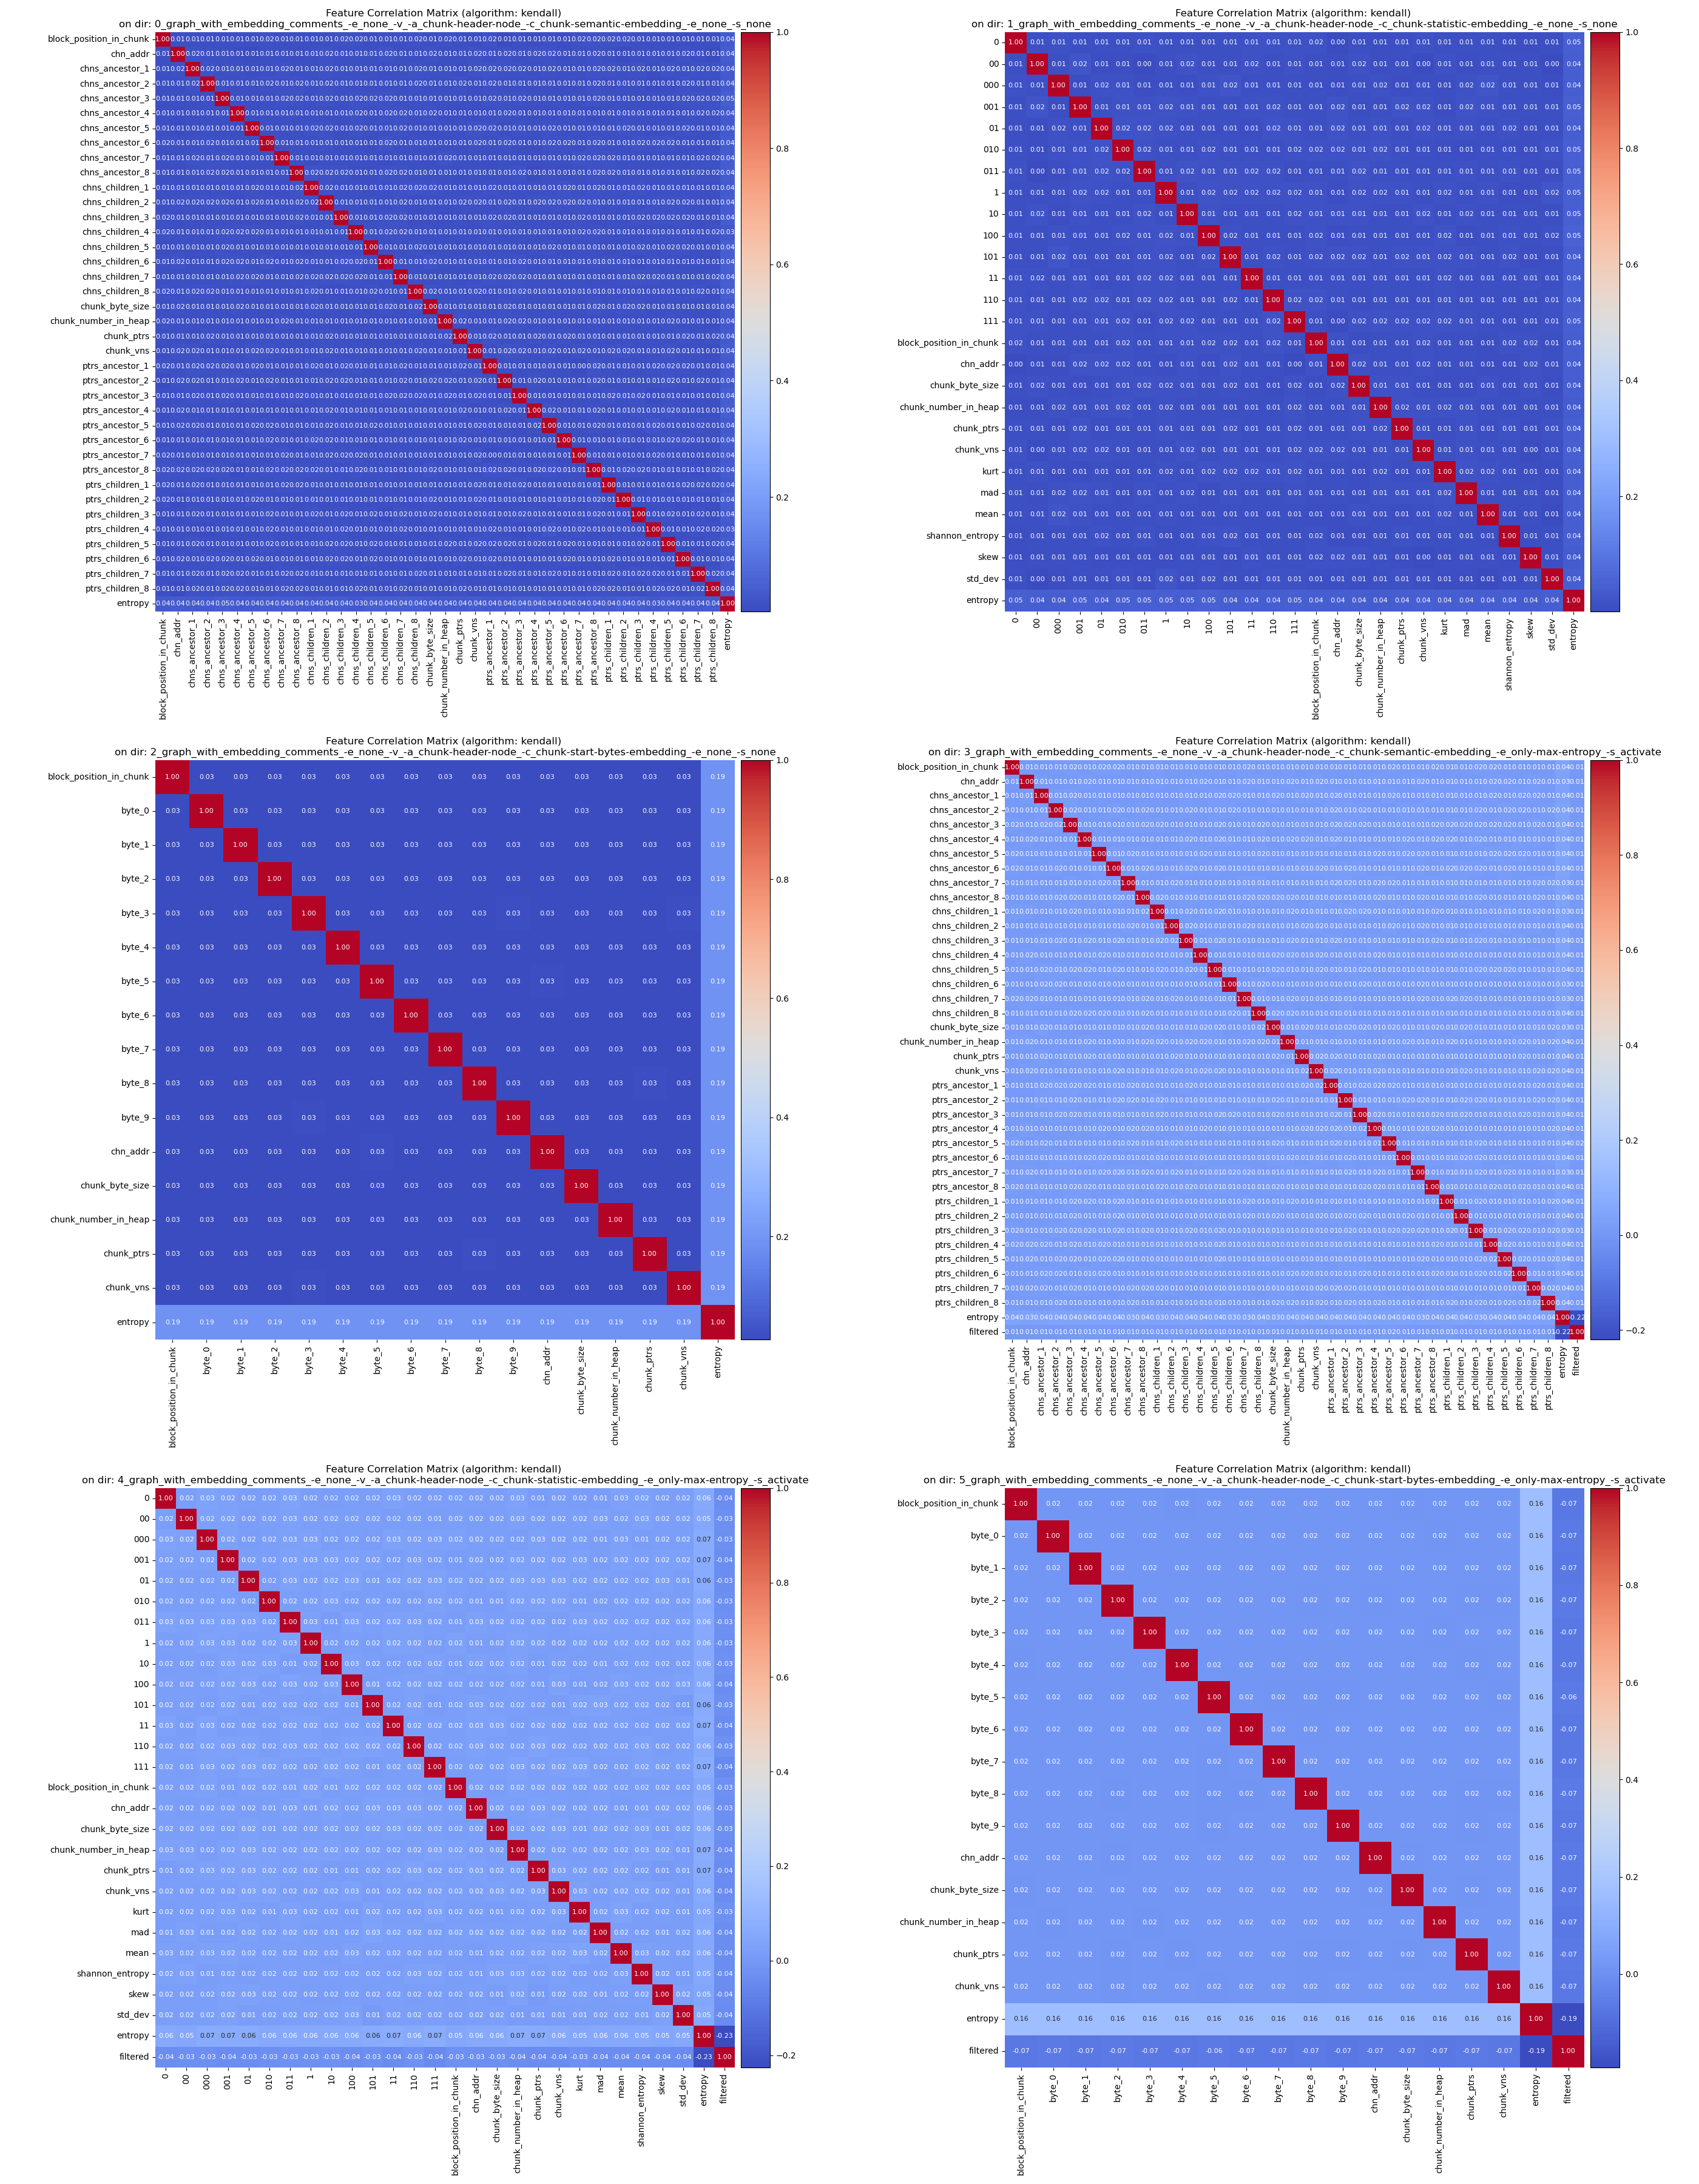
\includegraphics[width=16cm]{feature_engineering/concatenated_1_2023_10_24_kendall.png}
    \caption{Feature correlation matrices on the different Mem2Graph-generated datasets. Used algorithm: Kendall.}
\end{figure}

\begin{figure}[H]\label{results:corr_matrices:pearson}
    \centering
    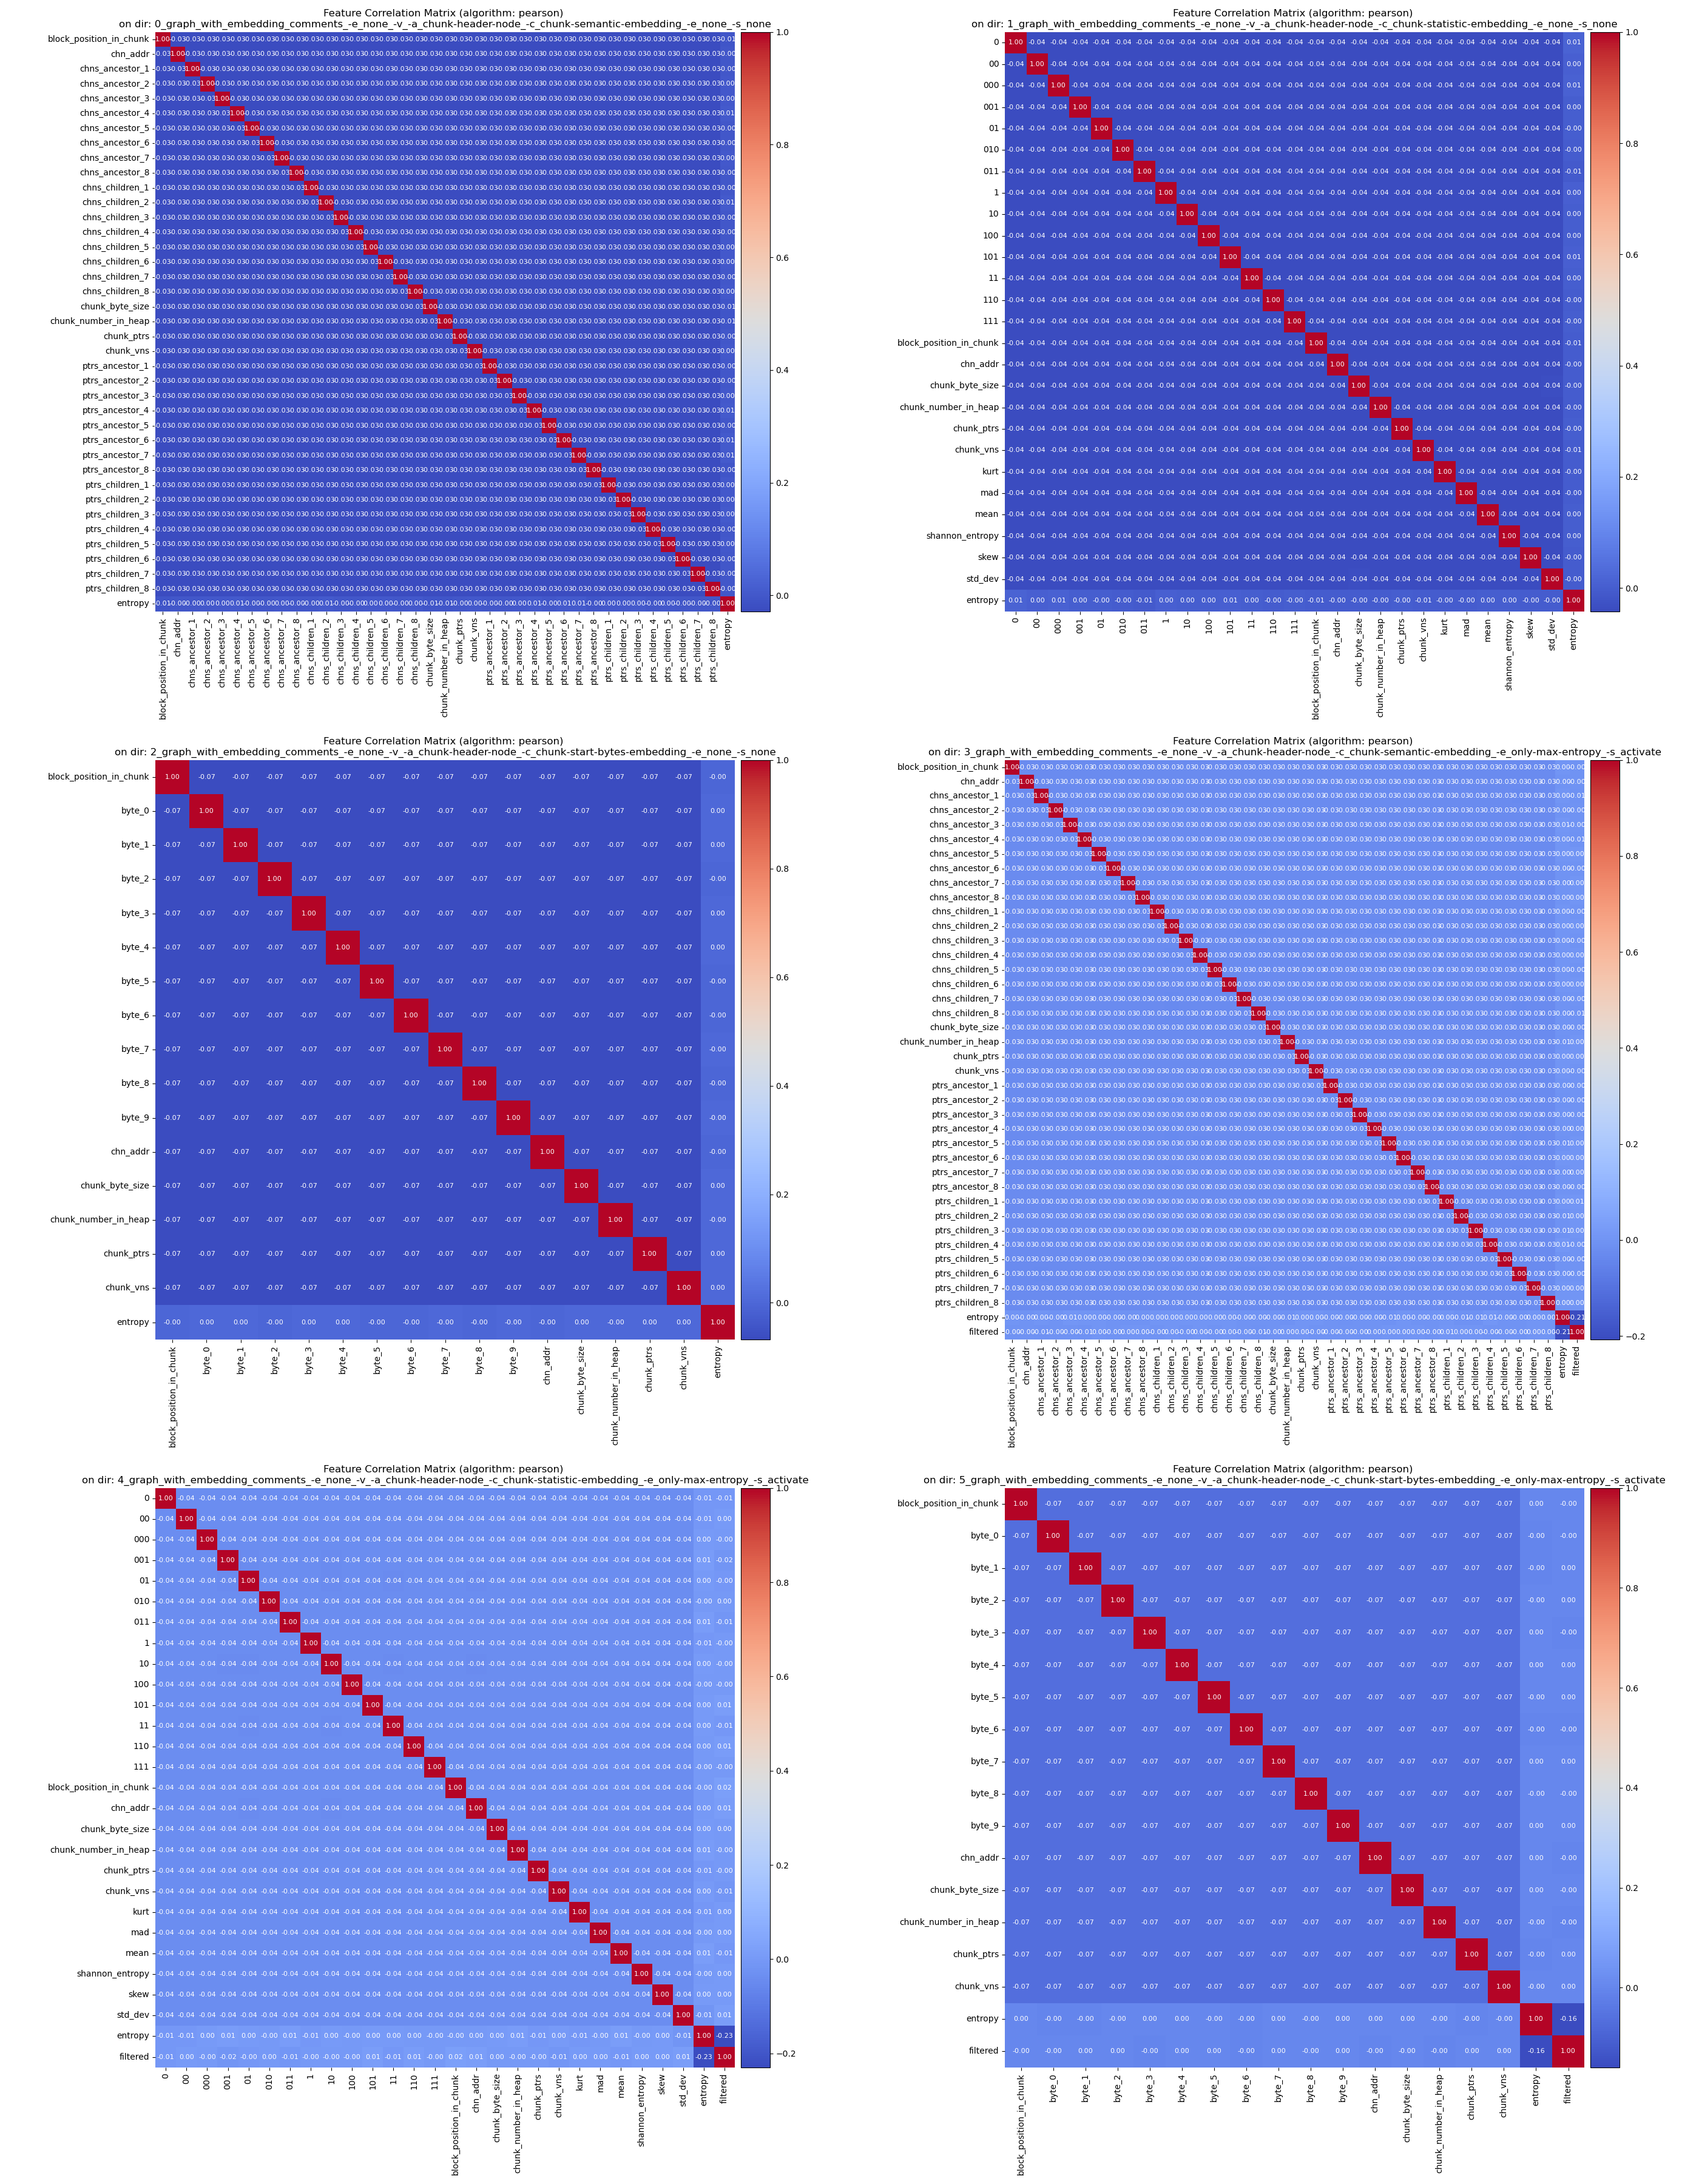
\includegraphics[width=16cm]{feature_engineering/concatenated_2_2023_10_24_pearson.png}
    \caption{Feature correlation matrices on the different Mem2Graph-generated datasets. Used algorithm: Pearson.}
\end{figure}

\begin{figure}[H]\label{results:corr_matrices:spearman}
    \centering
    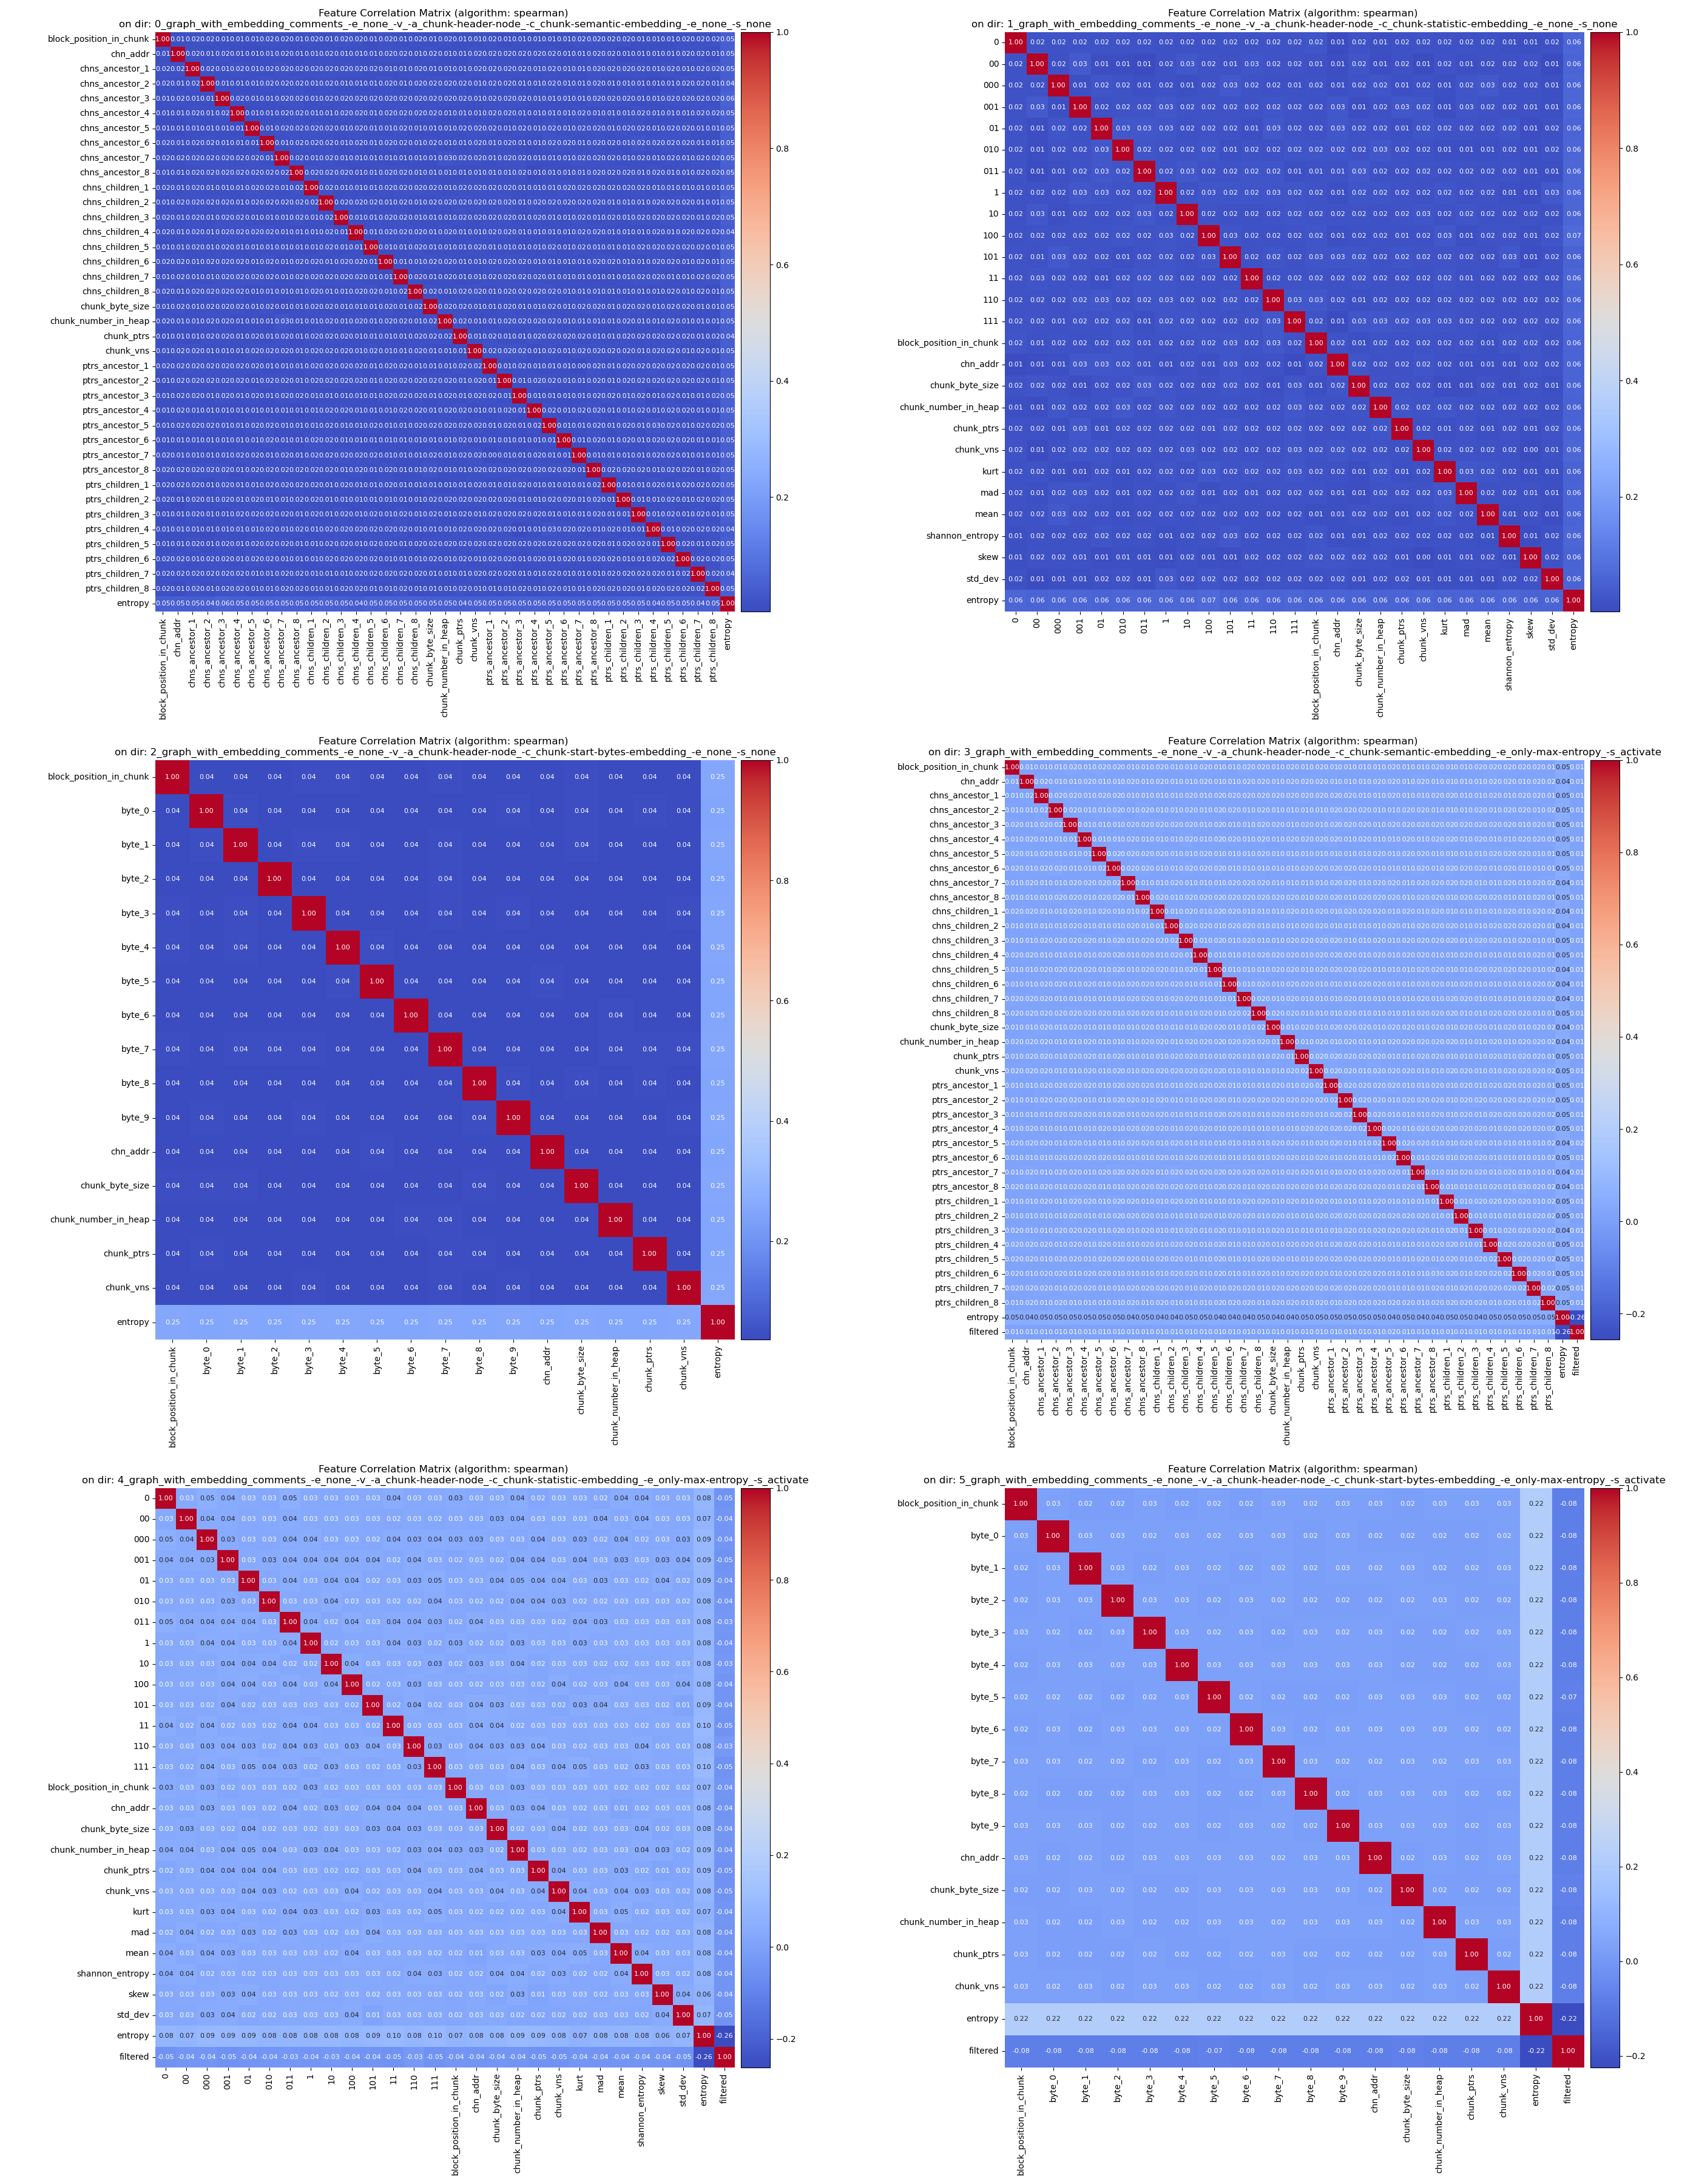
\includegraphics[width=16cm]{feature_engineering/concatenated_3__2023_10_24_spearman.png}
    \caption{Feature correlation matrices on the different Mem2Graph-generated datasets. Used algorithm: Spearman.}
\end{figure}

\subsection{Classic Model results}

Tables are provided to summarize the performance of different pipelines and models. These tables include four classical machine learning metrics: precision, recall, F1 score, and the Area Under the Curve (AUC). Each table offers a snapshot of how well each model performs on the key chunk prediction task.

\begin{table}[H]
    \centering
    \caption{Best instances of model: logistic-regression.}
    \begin{tabular}{lcccccc}
      \textbf{Best at}  & \textbf{Precision} & \textbf{Recall} & \textbf{F1 Score} & \textbf{AUC} \\
        precision & 1.0000 & 0.0417 & 0.0800 & 0.5208 \\
        recall & 0.3333 & 0.5000 & 0.4000 & 0.7471 \\
        f1 score & 0.3333 & 0.5000 & 0.4000 & 0.7471 \\
        AUC & 0.2449 & 0.5000 & 0.3288 & 0.7486 \\
    \end{tabular}
\end{table}


\begin{table}[H]
    \centering
    \caption{Best instances of model: random-forest.}
    \begin{tabular}{lcccccc}
      \textbf{Best at}  & \textbf{Precision} & \textbf{Recall} & \textbf{F1 Score} & \textbf{AUC} \\
        precision & 1.0000 & 0.0417 & 0.0800 & 0.5208 \\
        recall & 1.0000 & 0.0833 & 0.1538 & 0.5417 \\
        f1 score & 1.0000 & 0.0833 & 0.1538 & 0.5417 \\
        AUC & 1.0000 & 0.0833 & 0.1538 & 0.5417 \\
    \end{tabular}
\end{table}


\begin{table}[H]
    \centering
    \caption{Best instances of model: sgd-classifier.}
    \begin{tabular}{lcccccc}
      \textbf{Best at}  & \textbf{Precision} & \textbf{Recall} & \textbf{F1 Score} & \textbf{AUC} \\
        precision & 1.0000 & 0.0417 & 0.0800 & 0.5208 \\
        recall & 0.4615 & 1.0000 & 0.6316 & 0.9962 \\
        f1 score & 0.4615 & 1.0000 & 0.6316 & 0.9962 \\
        AUC & 0.4615 & 1.0000 & 0.6316 & 0.9962 \\
    \end{tabular}
\end{table}

\subsection{Deep Learning GCN Model results}
Best models obtained after the hyperparameter search, on a range of embeddings and models, this time focusing on the \acrshort{gcn} models.

\begin{table}[H]
    \centering
    \caption{Best instances of model: very-simple-gcn.}
    \begin{tabular}{lcccccc}
      \textbf{Best at}  & \textbf{Precision} & \textbf{Recall} & \textbf{F1 Score} & \textbf{AUC} \\
        precision & 0.6000 & 0.5000 & 0.5455 & 0.7489 \\
        recall & 0.2609 & 1.0000 & 0.4138 & 0.9907 \\
        f1 score & 0.6000 & 0.5000 & 0.5455 & 0.7489 \\
        AUC & 0.2609 & 1.0000 & 0.4138 & 0.9907 \\
    \end{tabular}
\end{table}

\begin{table}[H]
    \centering
    \caption{Best instances of model: simple-gcn.}
    \begin{tabular}{lcccccc}
      \textbf{Best at}  & \textbf{Precision} & \textbf{Recall} & \textbf{F1 Score} & \textbf{AUC} \\
        precision & 0.5000 & 0.5000 & 0.5000 & 0.7484 \\
        recall & 0.2308 & 1.0000 & 0.3750 & 0.9891 \\
        f1 score & 0.5000 & 0.5000 & 0.5000 & 0.7484 \\
        AUC & 0.2609 & 1.0000 & 0.4138 & 0.9907 \\
    \end{tabular}
\end{table}

\begin{table}[H]
    \centering
    \caption{Best instances of model: first-gcn.}
    \begin{tabular}{lcccccc}
      \textbf{Best at}  & \textbf{Precision} & \textbf{Recall} & \textbf{F1 Score} & \textbf{AUC} \\
        precision & 0.5000 & 0.5000 & 0.5000 & 0.7484 \\
        recall & 0.2727 & 1.0000 & 0.4286 & 0.9913 \\
        f1 score & 0.5000 & 0.5000 & 0.5000 & 0.7484 \\
        AUC & 0.2727 & 1.0000 & 0.4286 & 0.9913 \\
    \end{tabular}
\end{table}

\begin{table}[H]
    \centering
    \caption{Best instances of model: gcn-with-dropout.}
    \begin{tabular}{lcccccc}
      \textbf{Best at}  & \textbf{Precision} & \textbf{Recall} & \textbf{F1 Score} & \textbf{AUC} \\
        precision & 0.3500 & 0.2333 & 0.2800 & 0.6152 \\
        recall & 0.0863 & 0.8000 & 0.1558 & 0.8810 \\
        f1 score & 0.2110 & 0.7667 & 0.3309 & 0.8767 \\
        AUC & 0.0863 & 0.8000 & 0.1558 & 0.8810 \\
    \end{tabular}
\end{table}

\begin{table}[H]
    \centering
    \caption{Best instances of model: advanced-gcn.}
    \begin{tabular}{lcccccc}
      \textbf{Best at}  & \textbf{Precision} & \textbf{Recall} & \textbf{F1 Score} & \textbf{AUC} \\
        precision & 0.2097 & 0.4333 & 0.2826 & 0.7129 \\
        recall & 0.0533 & 0.9000 & 0.1006 & 0.8943 \\
        f1 score & 0.2097 & 0.4333 & 0.2826 & 0.7129 \\
        AUC & 0.1552 & 0.9000 & 0.2647 & 0.9390 \\
    \end{tabular}
\end{table}

\section{Compared Performances of models and embeddings}

In our experiments, we limited the analysis to a maximum of 16 input graphs, which may appear to be a relatively low number. However, this limitation was necessary due to the extensive range of hyperparameters, embeddings, and models that we aimed to evaluate. Despite this constraint, we were able to run a total of 7976 machine learning pipelines, accumulating over 100 hours of compute time. This extensive computational effort underscores the complexity and depth of the feature engineering and model evaluation processes undertaken in this study. The following tables and visualizations provide a comprehensive overview of the results obtained from these experiments.

\begin{table}[H]
    \centering
    \caption{Results for the model very-simple-gcn}
    \begin{tabular}{lcccccc}
      \textbf{Model}  & \textbf{Best Precision} & \textbf{Best Recall} & \textbf{Best F1 Score} & \textbf{Best AUC} \\
        advanced-gcn & 0.2097 & 0.9000 & 0.2826 & 0.9390 \\
        first-gcn & 0.5000 & 1.0000 & 0.5000 & 0.9913 \\
        gcn-with-dropout & 0.3500 & 0.8000 & 0.3309 & 0.8810 \\
        logistic-regression & 1.0000 & 0.5000 & 0.4000 & 0.7486 \\
        random-forest & 1.0000 & 0.0833 & 0.1538 & 0.5417 \\
        sgd-classifier & 1.0000 & 1.0000 & 0.6316 & 0.9962 \\
        simple-gcn & 0.5000 & 1.0000 & 0.5000 & 0.9907 \\
        very-simple-gcn & 0.6000 & 1.0000 & 0.5455 & 0.9907 \\
    \end{tabular}
\end{table}

In addition to the tabular data, we also offer visualizations to facilitate a more intuitive comparison between models and embeddings. These graphical representations aim to make the complex data more digestible and provide insights that may not be immediately obvious from the tables alone.

\begin{figure}[H]\label{results:compare:models:full}
    \centering
    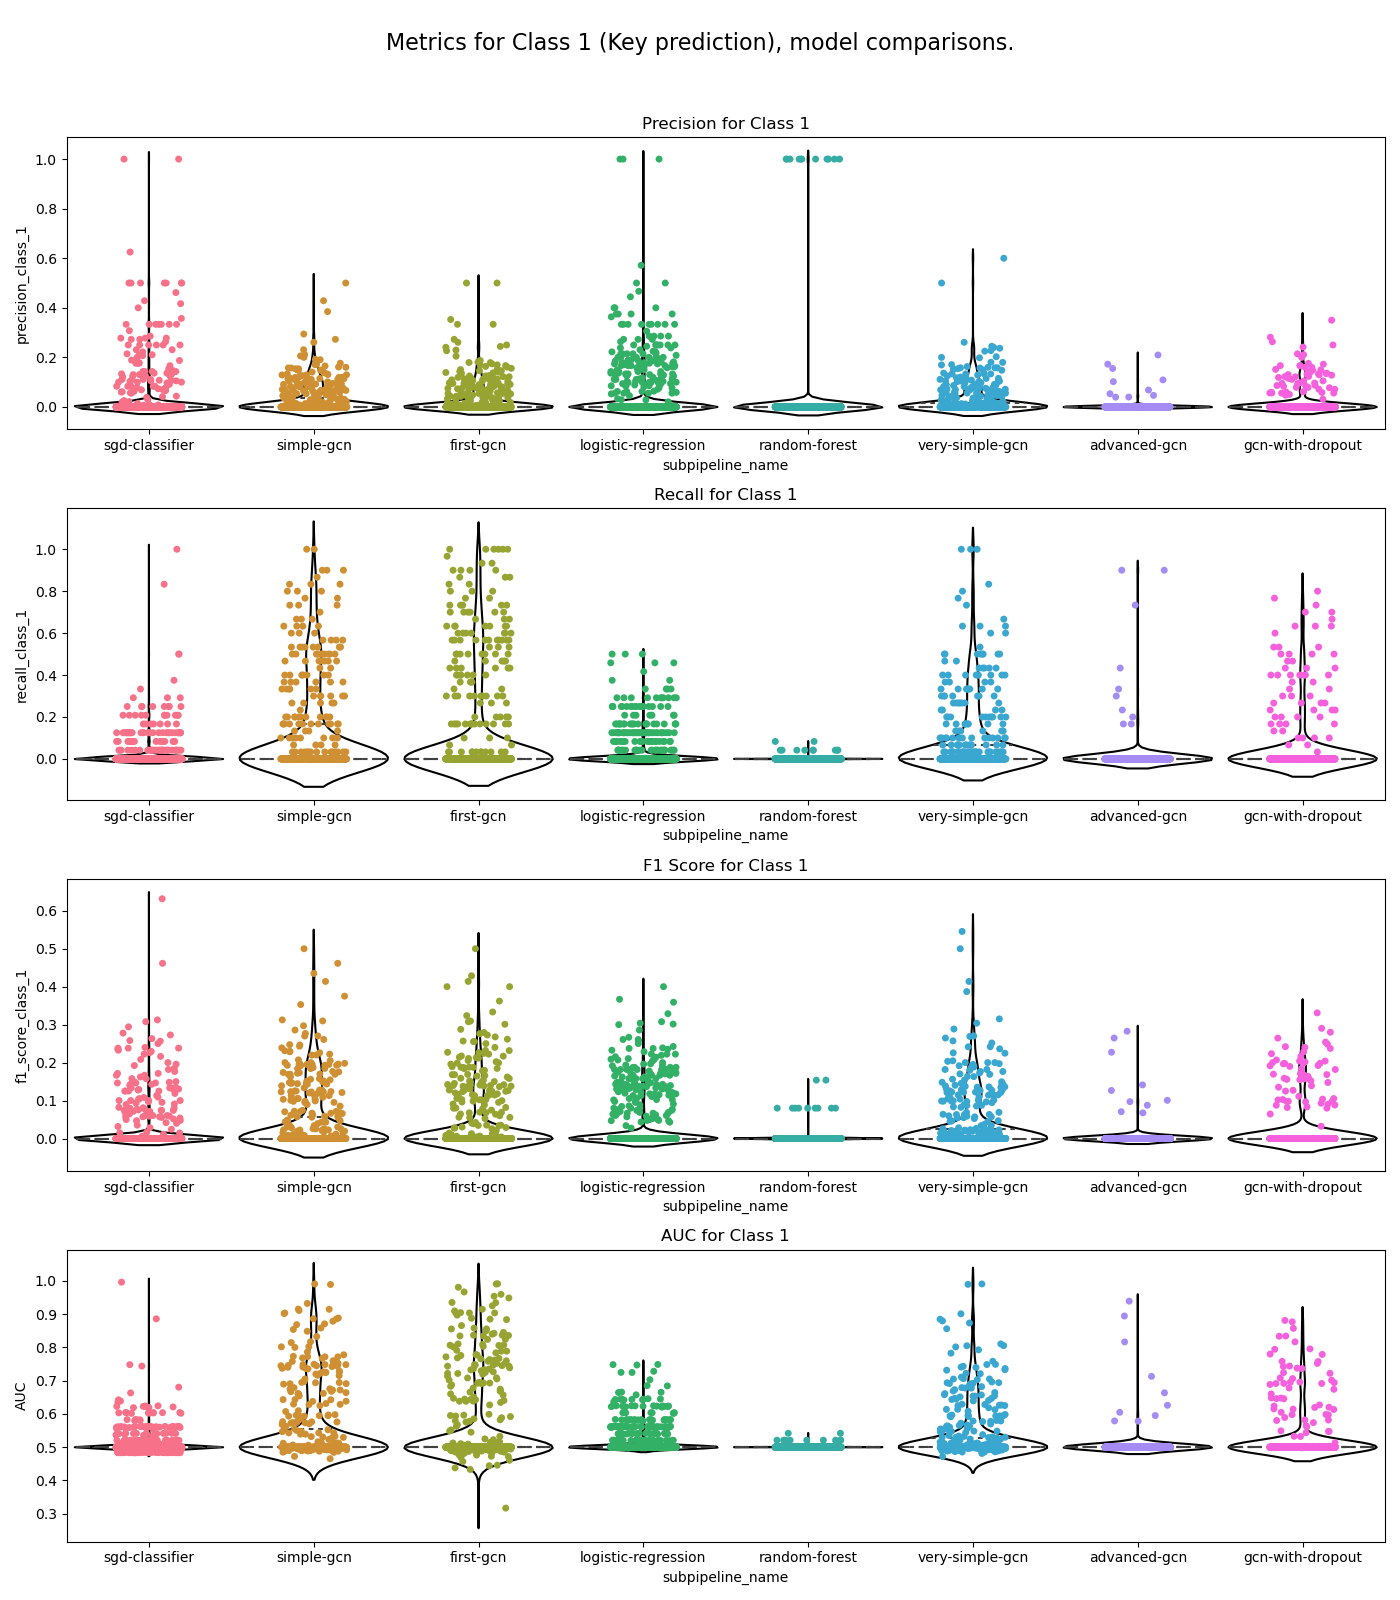
\includegraphics[width=16cm]{plots/models_comparison_metrics.png}
    \caption{Visualization of the result metrics use to compare model performance on memory graphs, for different embeddings and hyperparameters.}
\end{figure}

\begin{figure}[H]\label{results:compare:embeddings:full}
    \centering
    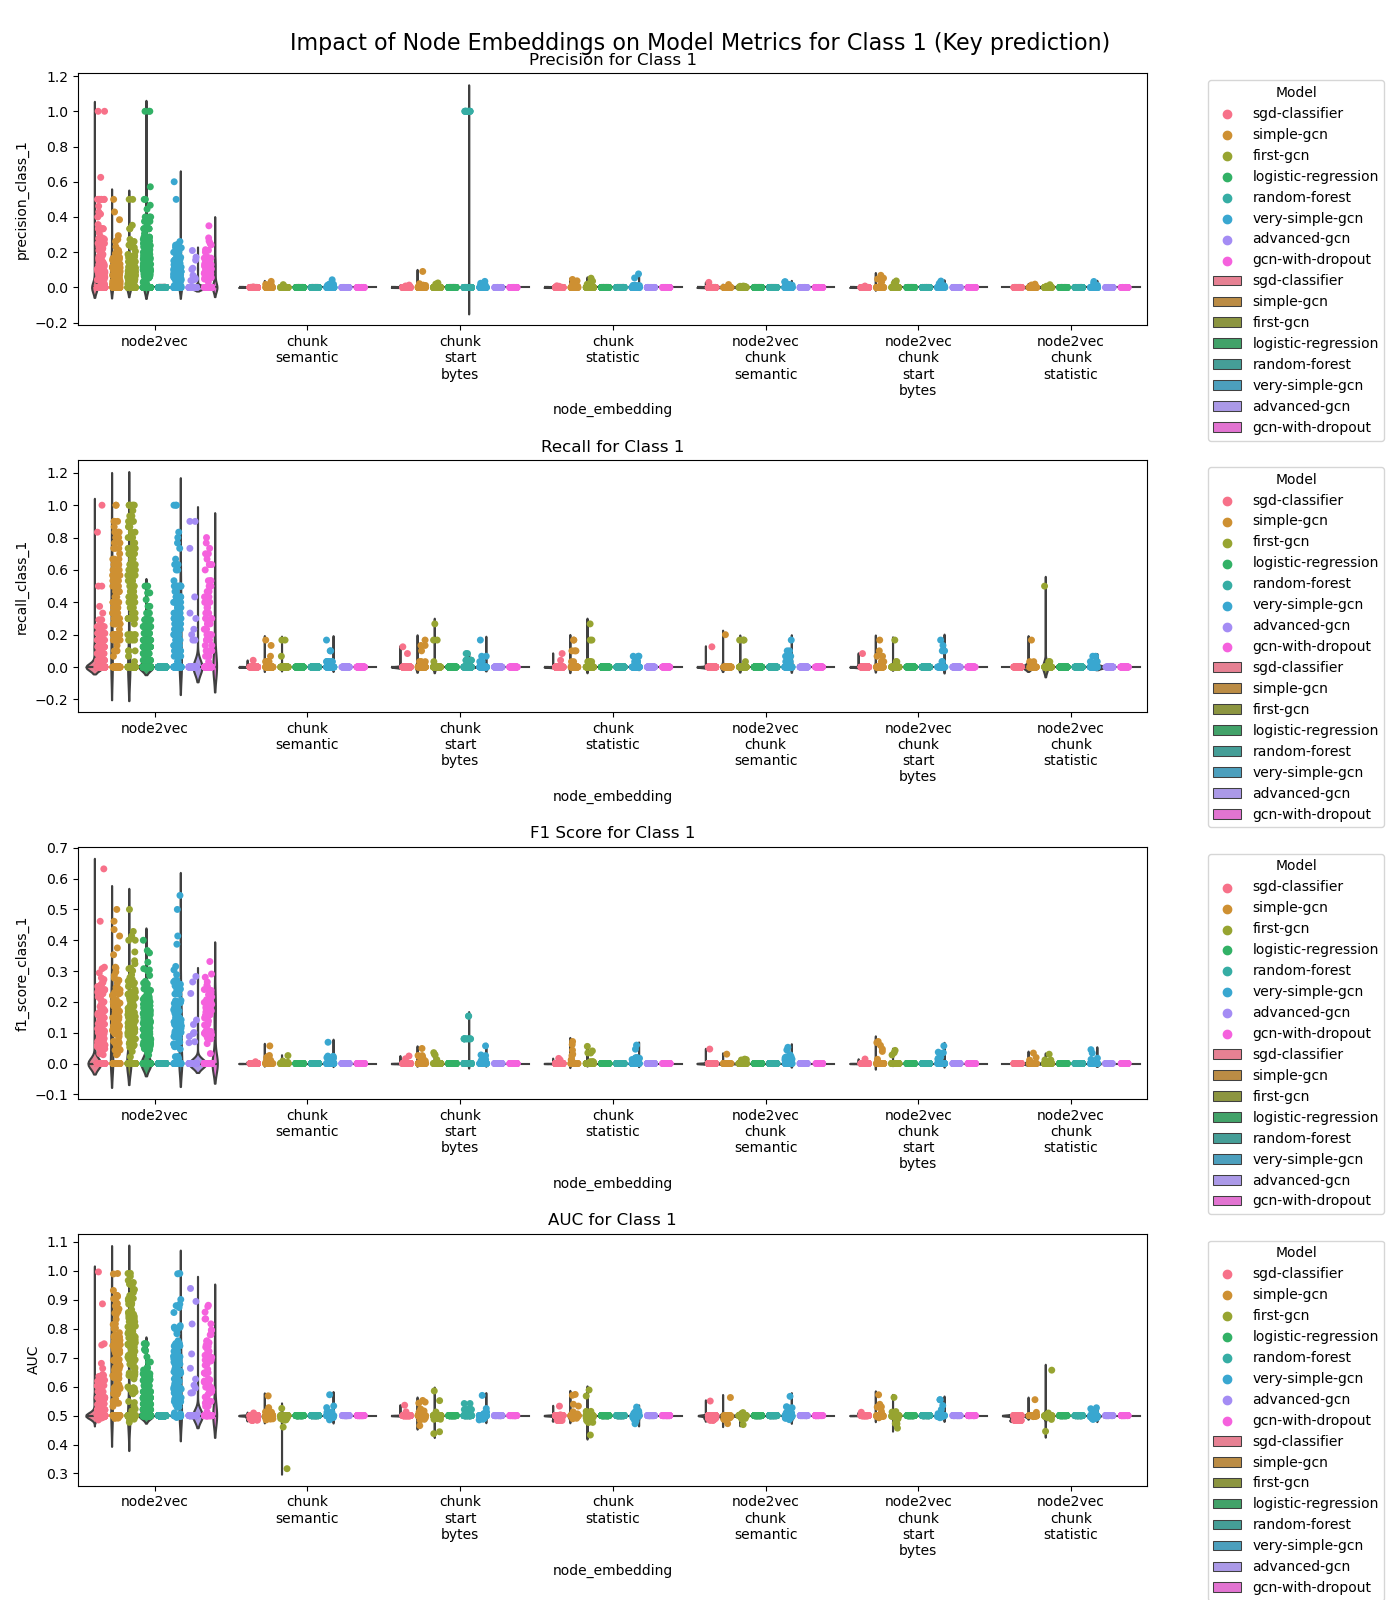
\includegraphics[width=16cm]{plots/embedding_comparison_metrics.png}
    \caption{Visualization of the result metrics use to compare model performance per memory graph node embedding strategies.}
\end{figure}

It's worth noting that while this section provides a detailed account of the results, an in-depth discussion about these findings, their implications, and potential future work will be covered in the following "Discussions" section.
